\documentclass[border=10pt]{standalone}
\usepackage{fontspec}
\setmainfont{DejaVu Sans}
\usepackage{tikz}
\usetikzlibrary{positioning, arrows.meta}

\begin{document}
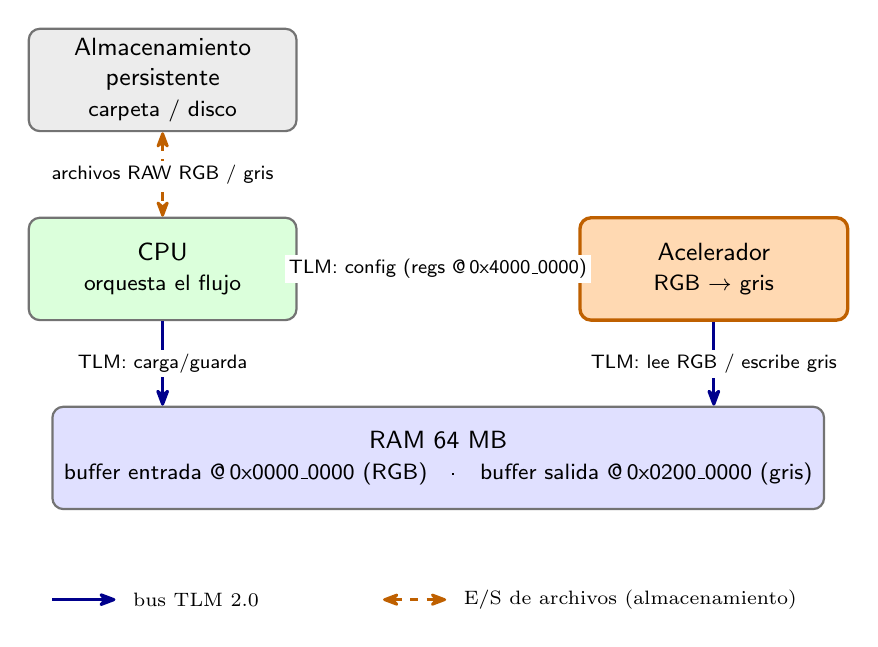
\begin{tikzpicture}[
  font=\sffamily\small,
  >={Stealth[round]},
  comp/.style={rectangle, rounded corners=4pt, draw=black!55, thick,
               minimum width=3.4cm, minimum height=1.3cm, align=center},
  tlm/.style={-{Stealth[round]}, line width=1.1pt, draw=blue!55!black},
  fio/.style={{Stealth[round]}-{Stealth[round]}, line width=1pt,
              draw=orange!75!black, dashed},
  lbl/.style={font=\sffamily\scriptsize, fill=white, inner sep=1.5pt},
]
% --- componentes ---
\node[comp, fill=gray!15]                                   (st)  at (0,4)   {Almacenamiento\\persistente\\{\footnotesize carpeta / disco}};
\node[comp, fill=green!14]                                  (cpu) at (0,1.6) {CPU\\{\footnotesize orquesta el flujo}};
\node[comp, fill=orange!30, draw=orange!75!black, line width=1.2pt]
                                                            (acc) at (7,1.6) {Acelerador\\{\footnotesize RGB $\to$ gris}};
\node[comp, fill=blue!12, minimum width=9.8cm]             (ram) at (3.5,-0.8)
      {RAM 64 MB\\{\footnotesize buffer entrada @\,0x0000\_0000 (RGB)\quad·\quad buffer salida @\,0x0200\_0000 (gris)}};

% --- conexiones ---
\draw[fio] (st) -- node[lbl]{archivos RAW RGB / gris} (cpu);
\draw[tlm] (cpu) -- node[lbl]{TLM: config (regs @\,0x4000\_0000)} (acc);
\draw[tlm] (cpu.south) -- node[lbl]{TLM: carga/guarda} (cpu.south |- ram.north);
\draw[tlm] (acc.south) -- node[lbl]{TLM: lee RGB / escribe gris} (acc.south |- ram.north);

% --- leyenda ---
\begin{scope}[shift={(-1.4,-2.6)}]
  \draw[tlm] (0,0) -- (0.8,0); \node[anchor=west, font=\scriptsize] at (0.9,0) {bus TLM 2.0};
  \draw[fio] (4.2,0) -- (5.0,0); \node[anchor=west, font=\scriptsize] at (5.1,0) {E/S de archivos (almacenamiento)};
\end{scope}
\end{tikzpicture}
\end{document}
